\documentclass[aspectratio=169]{beamer}
\usepackage{basileabeam}
\usepackage{comment}
\usepackage{amsfonts}
\usepackage{amsmath}

% Notes:
%\pgfpagesuselayout{2 on 1}[a4paper,border shrink=5mm]
%\setbeamertemplate{note page}[plain]
%\setbeameroption{show notes on second screen=bottom}

\title              {Mutex Based Potential Heuristics}

\author             {Salome M\"uller}
\email              {salo.mueller@unibas.ch}
\institute          {Department of Mathematics and Computer Science, University of Basel}

\date               {20.11.2020}

\ulogo                {Template/header}
\ulistelement        {Template/listelement}

\graphicspath{{Figures/}}

% Options:
\totalNoSlidesDisabled % To turn off the total number of slides in the footer. Comment this if you want the total number of slides in the footer

%\headerSectionsDisabled % Comment this if you want a fancy header containing your sections.


\begin{document}

    \begin{frame}[t,plain]
        \titlepage
    \end{frame}

    \note{Notes can help you to remember important information. Turn on the notes option.}

    \section{Background}

    \begin{frame}[c]{Classical Planning}
        \begin{itemize}
            \item States $s\in\mathcal{S}$
            \item Facts $f = \langle V, v  \rangle$, $f\in\mathcal{F}$
            \item Operators $o\in\mathcal{O}$
                \begin{itemize}
                    \item $\text{cost}(o)$
                    \item $\text{pre}(o)\subset\mathcal{F}$
                    \item $\text{eff}(o)\subset\mathcal{F}$
                \end{itemize}
        \end{itemize}
    \end{frame}

    \begin{frame}[c]{15-Puzzle}
        \begin{figure}
            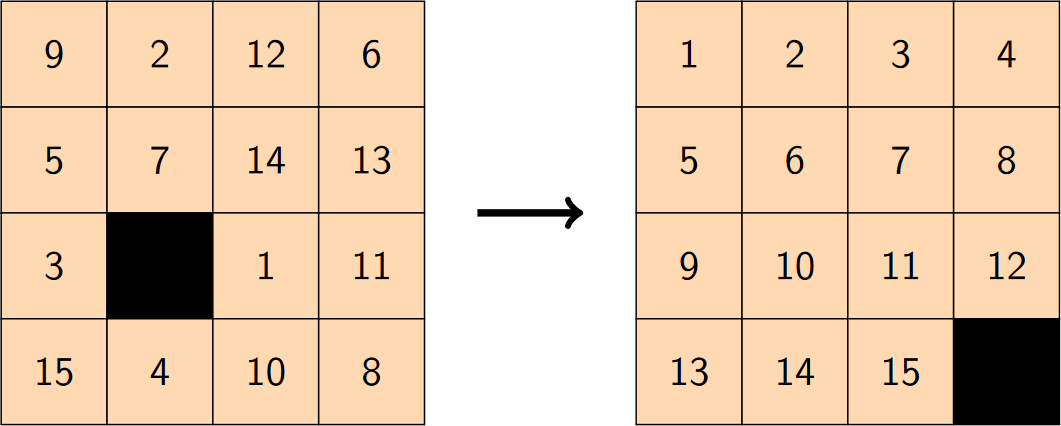
\includegraphics[width=0.8\textwidth]{15-puzzle}
        \end{figure}
        \begin{columns}[c]
            \column{.5\textwidth}
            \center Initial State
            \column{.5\textwidth}
            \center Goal State
        \end{columns}
    \end{frame}

    \begin{frame}[c]{Potential Heuristics}
        \[h:\mathcal{R} \rightarrow \mathbb{R} \cup \{\infty\}\]
        \newline
        \[h^\mathtt{P}(s)=\sum_{f\in s}P(f)\]
    \end{frame}

    \begin{frame}[c]{Linear Program}
        \begin{itemize}
            \item Optimization Functions
                \begin{itemize}
                    \item Linear combination of potentials
                    \item Different heuristic for different Optimization Functions
                \end{itemize}
            \item Constraints
                \begin{itemize}
                    \item Inequalities
                    \item Assure properties
                \end{itemize}
        \end{itemize}
    \end{frame}

    \begin{frame}[c]{Mutexes}

    \end{frame}

    \section{Optimization Functions}
    \begin{frame}[c]{Mutex Based Potential Heuristics}
        Mention all states potential heuristic (all syntactic states). Upper bound on appearance of fact.
        Insert CKF (?), Explain that strengthening results in new, lower upper bound, mention weights.
        (opt functions on backup slides)
        Introduce ensemble hueristics, mention that we do it by starting with partial state of size |t|, state random, one state = one heuristic.
    \end{frame}

    \begin{frame}[c]{Optimization Functions: Results}
         Table with all + 3 mutex based (+ or Plot ?) or only coverage.
         Take 1-2 bullet points from evaluation.
    \end{frame}


    \section{Linear Program}
    \begin{frame}[t]{Strenghten Constraints}
        Constraints invovled all facts, now they only involve facts which are possible, as they do not influence this operator.
        Formulas on backup slides
    \end{frame}

    \begin{frame}[t]{Strenghten Constraints: Results}
        Table with 2-3 unstrengthened + 2-3 strengthened. or Plot. or only coverage.
        Take 1-2 bullet points from evaluation.
        Max.
    \end{frame}


    \section{Additional Constraints}
    \begin{frame}[c]{Additional Constraints}
        Basic idea.
        \[\sum_{f\in s}\mathtt{P}(f)=h^\mathtt{P}(s)\]
        For initial and for random states, explain how random states are generated.
    \end{frame}

    \begin{frame}[c]{Additional Constraints: Results}
        Table with 2-3 unstrengthened + 2-3 strengthened. or Plot. or only coverage.
        Take 1-2 bullet points from evaluation.
        Max?
    \end{frame}

    \section{Conclusion}
    \begin{frame}[t]{Conclusion}
        Good, but to slow, computationally expensive as implemented.
        1-2 Bullet points from conclusion, on conclusions and bullet points.
    \end{frame}


    \begin{frame}[t,plain]
        \lastpage{{\usebeamerfont{title} Questions?}\\[5ex]
        salo.mueller@unibas.ch}
    \end{frame}

    \backupbegin

    \begin{frame}[c]{Theorem}
        Now we introduce an equation.
        \begin{theorem}
            A Turing Machine is a 7-Tuple:
            \begin{equation}
                M = \langle Q, \Gamma, b, \Sigma, \delta, q_0, F \rangle
            \end{equation}
        \end{theorem}
        A Turing Machine is a 7-Tuple even if defined in the text, as in $M = \langle Q, \Gamma, b, \Sigma, \delta, q_0, F \rangle$.
    \end{frame}

    \backupend

\end{document}

